\documentclass[10pt,twocolumn]{article} 
\usepackage{simpleConference}
\usepackage{times}
\usepackage{graphicx}
\usepackage{amssymb}
\usepackage{url,hyperref}
\usepackage[font=small,labelfont=bf]{caption}
\usepackage{amsmath}
\usepackage{booktabs}

\begin{document}

\title{Empirical convergence analysis for radial basis functions (RBF) and polynomial feature selection on episodic semi-gradient TD(0)}

\author{Bonetti, Mauricio L.\\
mauricio@codecraftit.com\\
February 21, 2024 \\
}

\maketitle
\thispagestyle{empty}

\begin{abstract}
Temporal difference (TD) learning has been used to learn strong evaluation functions in a variety of scenarios. In this paper we compare the convergence obtained 
by applying radial basis functions (RBF) and polynomial feature selections on episodic semi-gradient TD(0) to solve 
a well-studied benchmarking problem, namely the "mountain-car" problem, which challenge the model with large 
and continuous input space. Different models were trained with a range of discounting. Convergence analysis is exposed based 
on the number of training sessions required for reaching convergence and the statistics of the amount of steps needed to complete the task.
\\ \\\textbf{Keywords:} Reinforcement Learning, Temporal Difference Learning, Mountain Car, Markov Chain, Function Approximation, Radial Basis Function, Polynomial Feature Selection
\end{abstract}

\section{Introduction and Background}
Learning algorithms have the potential to reduce the difficulty of building and
tuning complex systems. But, there is often a significant amount of work required
to tune each learning approach for specific problems and domains. \cite{Feature_Construction}
The problem selected for this research was extracted from \cite{Sutton1998} and is defined as follows:
Consider the task of driving an underpowered car up a steep mountain road, The difficulty is that gravity is stronger
than the car’s engine, and even at full throttle the car cannot accelerate up the steep slope.
Many control methodologies have great difficulties with tasks of this kind unless explicitly aided by a
human designer. The reward in this problem is (-1) on all time steps until the car moves past its goal
position at the top of the mountain, which ends the episode. There are three possible
actions: full throttle forward (+1), full throttle reverse (-1), and zero throttle (0). 

\begin{figure}
  \begin{center}
      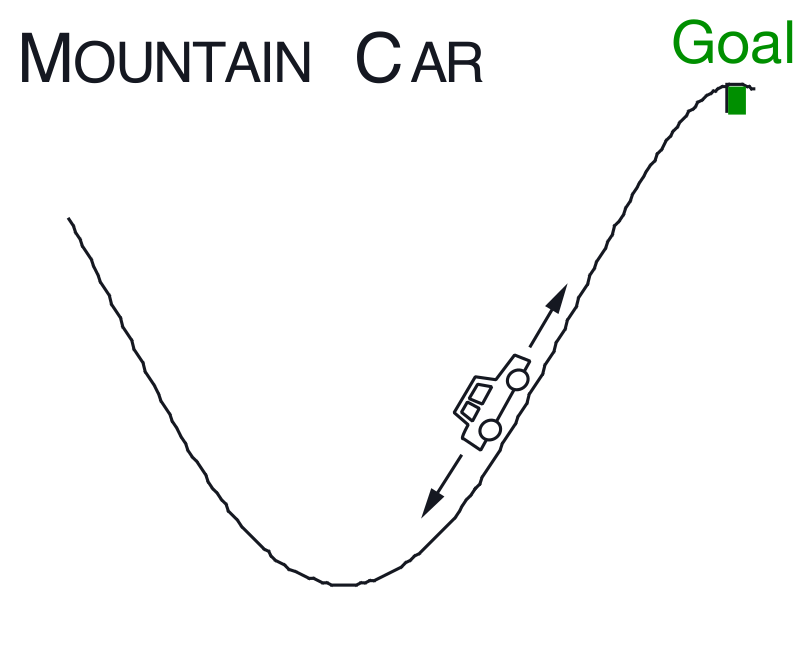
\includegraphics[scale=0.2]{mountain-car.png}
  \end{center}
  \caption{The Mountain Car task. Drawing from \cite{Sutton1998}}.
  \label{mountain_car}
\end{figure}

The car moves according to a simplified physics. The car's position ($p_{t}$) and its velocity ($v_{t}$) is updated by the following equations:
\\ \\
$p_{t+1} = p_{t} + v_{t+1}$
\\
$v_{t+1} = v_{t} + 0.001A_{t} - 0.0025cos(3p_{t})$
\\ \\
Where $p_{t}\in[-1.2,0.5]$, $v_{t}\in[-0.07,0.07]$ and $A_{t}\in\{-1, 0, 1\}$. An extensive discussion regarding the physics background of the mountain-car problem can be found in \cite{Mountain}. We decided to train an on-policy model for this control problem
using $\epsilon-greedy$ for action selection with parametric approximation of the action-value function $\hat{q}(s, a, w) \approx q_*(s,a)$ where $w\in\mathbb{R}^d$ is a finite-dimensional weight vector.


\section{Episodic Semi-gradient Sarsa}
Semi-gradient Sarsa algorithm is the natural extension of semi-gradient TD(0) to action values and to on-policy
control. \cite{Sutton1998} In this paper, for convenience, we refer to this algorithm as TD(0). Given the information of position and velocity we build feature vectors $\mathbf{x}(s,a)$ 
and combine them linearly with the weight vector $\mathbf{w}$ as follows:
\\ \\
$\hat{q}(s, a, \mathbf{w}) = \mathbf{w}^T \mathbf{x}(s,a) = \sum_{i=1}^{d} w_i . x_i(s,a)$
\\ \\
And the gradient-descent update for action-value is defined by:
\\ \\
$\mathbf{w}_{t+1} = \mathbf{w}_{t} + \alpha[R_{t+1} + \gamma \hat{q}(S_{t+1}, A_{t+1}, \mathbf{w}) - \hat{q}(S_{t}, A_{t}, \mathbf{w})] \nabla \hat{q}(S_{t}, A_{t}, \mathbf{w})$
\\ \\
A temporal difference model (TD) becomes a potential solution for this problem due to the problem characteristic of having a limited set of distinct actions that can be taken. 
Each action will have its own associated weight vector $\mathbf{w}$ such that:
\[
\hat{q}(s, a, \mathbf{w}) = \begin{cases}
  \mathbf{w}_{-1}^T \mathbf{x}(s,a) & \text{if \(a\) = -1} \\
  \mathbf{w}_{0}^T \mathbf{x}(s,a) & \text{if \(a\) = 0} \\
  \mathbf{w}_{1}^T \mathbf{x}(s,a) & \text{if \(a\) = 1} \\
\end{cases}
\]
Policy improvement is done by changing the estimation policy to a soft approximation of the greedy policy ($\epsilon-greedy$), the selected action $A_{t}$ is defined by:
\[
A_{t} = \begin{cases}
  {argmax}_{a} \hat{q}(S_{t}, A_{t}, \mathbf{w}) & \text{with probability = (1 - $\epsilon$)} \\
  {random}_{a} & \text{otherwise} \\
\end{cases}
\]
Convergence proof can be found in \cite{QLearning}. 
We are considering \emph{training session} the process of updating the weights based on TD(0) starting from a random position $p_{0}\in[-0.6,-0.4]$ having $v_{0} = 0$. 
In order to obtain a satisfactory convergence rate, each \emph{training session} is configured with a set of parameters $\alpha$, $\gamma$, $\epsilon$, \emph{polynomial dimension} (for polynomial model) and \emph{proto points} (for RBF)
. where $\alpha \in \{0.010, 0.025, 0.05, 0.075, 0.1, 0.125, 0.150, 0.175, 0.2, 0.4,\\ 0.5\}$, $\gamma \in \{0.8, 0.9, 0.95, 0.99, 1.0\}$,
 $\epsilon \in \{0.25, 0.5, 0.75\}$, $\emph{polynomial dimension} \in \{2, 3, 4, 5, 6, 7, 8, 9, 10\}$, $\emph{proto points per dimension} \in \{8, 12, 18, 21, 27, 36, 52\}$. 
 Each training session runs 500 episodes. An episode terminates when the final position $p_{f} = 0.5$ is reached or when the amount of steps taken so far exceeds 5000 (non-converging).
 Once a \emph{training session} is completed we ran 1000 simulations with the trained model starting again from a random position $p_{0}\in[-0.6,-0.4]$ having $v_{0} = 0$. 
 If every simulation reaches the final position and the mean of steps needed to complete the task in the 1000 simulations is below 300, then we are considering that
  a satisfactory convergence was reached. 

\subsection{Polynomial Feature Selection}
The state space in the "mountain-car" problem is expressed in numbers, in this type of problem, function approximation for reinforcement
learning has much in common with the familiar tasks of interpolation and regression. Various families of features commonly used 
for interpolation and regression can also be used in reinforcement learning. Polynomials make up one of the simplest families of
features used for interpolation and regression. \cite{Sutton1998} Considering the physics of the problem it is immediate to identify
the relationship between position and velocity. Higher-dimensional feature vectors take more complex interactions into account.
To generate the features, variables were scaled and translated individually by the given range on the training set using Min-Max \cite{Normalization}:
\\ \\
$p_{scaled} = (p - p_{min}) / (p_{max} - p_{min}$)
\\
$v_{scaled} = (v - v_{min}) / (v_{max} - v_{min}$)
\\ \\
Where $p_{min} = -1.2$, $p_{max} = 0.5$, $v_{min} = -0.07$, $v_{max} = 0.07$. With scaled variables, we can represent highly-complex interactions among state
dimensions. For this 2-dimensional state space, each order-$n$ polynomial-basis feature $x_i$ can be written as:
\\ \\
$x_{i}(s) = \prod_{j=1}^{2} s_{j}^{c_{i,j}}$
\\ \\
where each $c_{i,j}$ is an integer in the set $\{0, 1, .. , n\}$ for an integer $n = \emph{polynomial dimension}$. These
features make up the order-n polynomial basis for dimension 2, which contains $(n + 1)^2$ different features. \cite{Sutton1998}

\subsection{RBF Feature Selection}
Radial Basis Functions is a technique for interpolating in a high dimensional space, it constructs a linear function space which depends on
the positions of the known data points (proto points) according to an arbitrary distance measure. \cite{Radial}. For this research we have adopted the parametrization
$\emph{proto points per dimension}$. To illustrate the proto points distribution, if we set $\emph{proto points per dimension} = 3$, and knowing we have two dimensions
(position and velocity) in this problem, then we will have the proto points distributions as shown in figure [\ref{rbf-figure}].
\begin{figure}[h]
  \begin{center}
      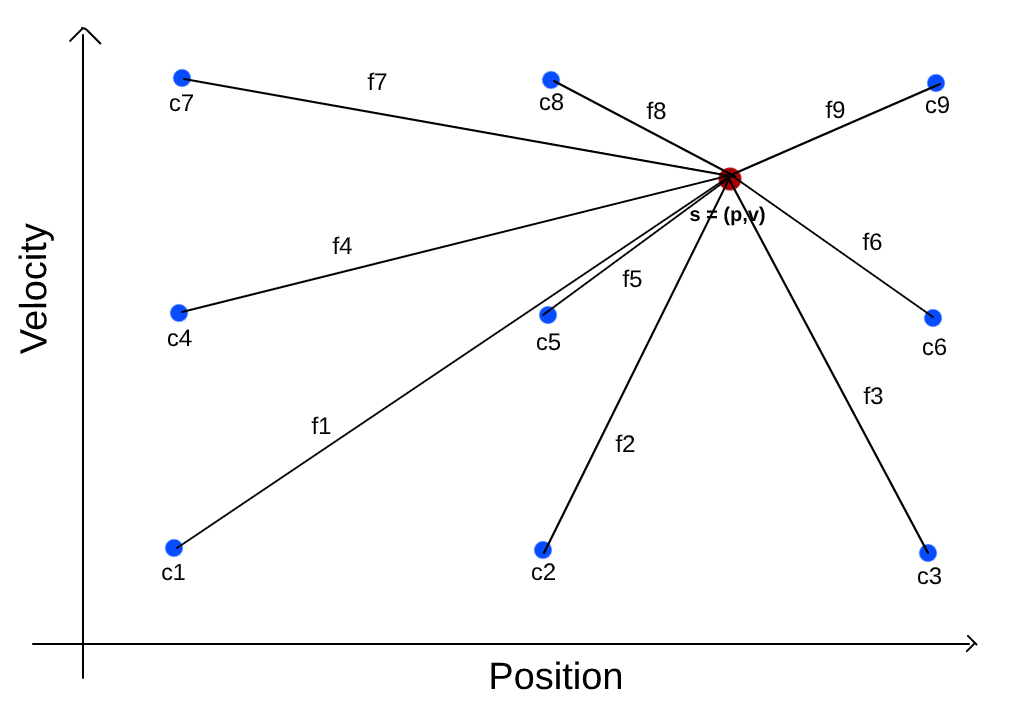
\includegraphics[scale=0.2]{rbf.png}
  \end{center}
  \caption{Interpolation for 3 proto points per dimension for state $s$. The distances $f_{i}$ are the features to be trained.}
  \label{rbf-figure}
\end{figure}
The smoothness of a Gaussian RBF is controlled by the magnitude of distance scaler $\sigma$. In this research we have applied:
$\mathbf{\sigma} = \begin{bmatrix} 1.7 * \emph{scaler} \\ 0.14 * \emph{scaler} \end{bmatrix}$. Where $\emph{scaler} = 0.005$. 
The constant factors are the differences between the maximum and minimum limits for position and velocity. RBF is defined as follows:
\\ \\
$\varphi(\mathbf{x_{t}}, \mathbf{c}) = exp(-(|| \mathbf{x_{t}} - \mathbf{c} ||^2 / \mathbf{\sigma}))$
\\ \\
Where $\mathbf{c}$ is the proto points vector and $\mathbf{x_{t}}$ is the vector representing the state (position and velocity) at a given time $t$.


\section{Convergence Analysis for Polynomial}
Considering the variations in discountings ($\alpha$, $\gamma$, $\epsilon$) and $\emph{polynomial dimension}$ ranging from 2 to 10, we trained a total of 1,485 models, 
 assuming each model underwent 10 training sessions, we conducted 14,850 training sessions for polynomial feature selection. From these, 121 training sessions converged (0.81\%).
  Inspecting the converging polynomial models we have observed that it was possible to reach convergence on every $\emph{polynomial dimension}$ from selected range. The distribution is exposed in the histogram [\ref{histogram_polynomial_convergent_training_sessions}]. 
  Notice that 17.36\% of convergent training models have $\emph{polynomial dimension} = 5$, indicating this might be the dimension having the best convergence rate in the selected range. 
  The table [\ref{polynomial-convergence-result}] reveals the count of training sessions necessary to achieve convergence for each set of discountings utilized,
  we selected the models with highest convergent rate only. Considering every convergent model, the average of training session required to reach convergence was 1.26 (12.60\% of training sessions). 
  We performed 1000 simulations for each convergent model, and table [\ref{polynomial-simulation-result}] showcases the minimum and maximum trajectory sizes, 
along with their corresponding statistics. A convergent model trained with $\emph{polynomial dimension} = 4, \alpha = 0.075, \gamma = 0.99, \epsilon = 0.75 $ while running the simulations has generated trajectory sizes 
with standard deviation of 2.03 steps revealing a strong consistency of the model on solving the problem. 
  The graph [\ref{means_of_trajectory_sizes_for_polynomial_convergent_models}] illustrates the mean of the averages of trajectory sizes computed for each $\emph{polynomial dimension}$. 
  The convergent models for $\emph{polynomial dimension} = 7$ provided the smallest mean of trajectory size, the calculated mean for this experiment was 147 steps. The convergent model with a $\emph{polynomial dimension} = 2$ stands out as the one with the smallest 
  set of features among all convergent models (totaling $(2 + 1)^2 = 9$ features). Throughout the 1000 simulations conducted for the models having $\emph{polynomial dimension} = 2$, 
  the maximum trajectory size observed was 306, with a mean of 220.94 and a standard deviation of 36.  

\begin{figure}[t]
  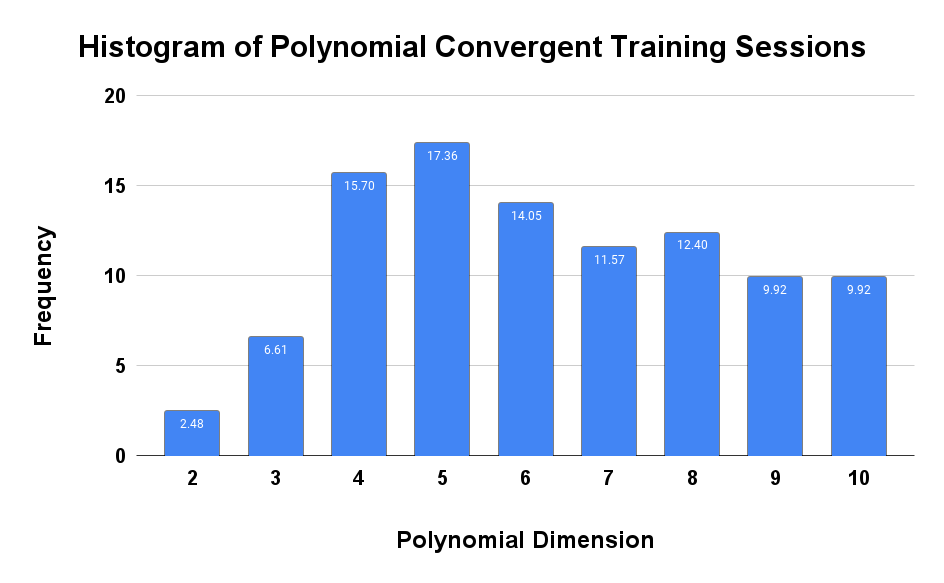
\includegraphics[scale=0.25]{histogram-polynomial-convergent-training-sessions.png}
  \caption{Histogram of Polynomial Convergent Training Sessions.}
  \label{histogram_polynomial_convergent_training_sessions}
\end{figure}

\begin{figure}[t]
  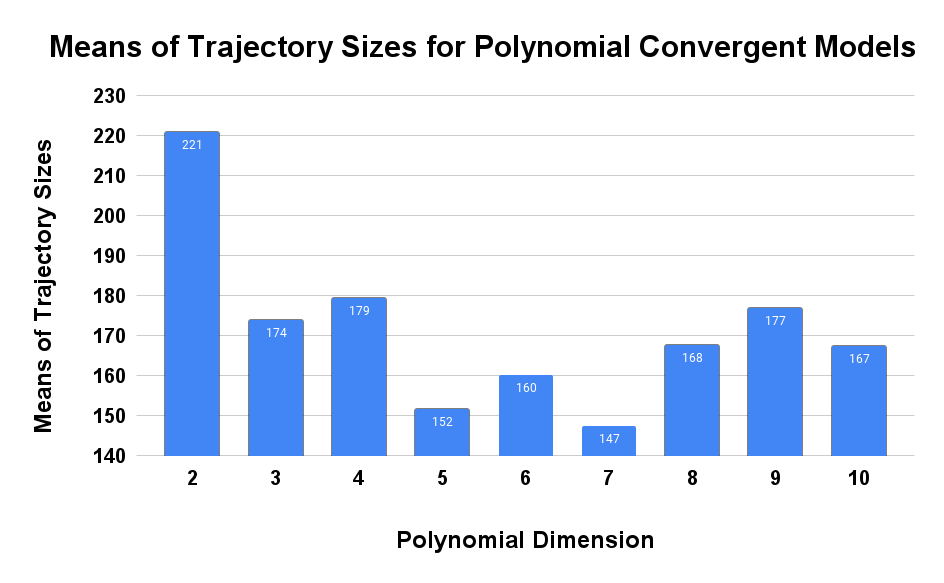
\includegraphics[scale=0.25]{means-of-trajectory-sizes-for-polynomial-convergent-models.png}
  \caption{These represents the means of the averages of trajectories sizes obtained from each convergent model, considering the entire set of discoutings applied.}
  \label{means_of_trajectory_sizes_for_polynomial_convergent_models}
\end{figure}


\section{Convergence Analysis for RBF}
The same discountings were used for RBF feature selections ($\alpha$, $\gamma$, $\epsilon$), and $\emph{proto points per dimension} \in \{8, 12, 18, 21, 27, 36, 52\}$.  
We trained a total of 1,155 models and considering each model underwent 10 training sessions, we conducted 11,550 training sessions for the RBF feature selection. 
From these, 4,631 training sessions converged (40.09\%). Inspecting the converging RBF models we have observed that it was possible to reach convergence on every $\emph{proto points per dimension}$ from selected range.
The distribution is exposed in the histogram [\ref{histogram_rbf_convergent_training_sessions}]. Notice that 21.79\% of convergent training models have $\emph{proto points per dimension} = 12$, indicating this might be the dimension having the best convergence rate in the selected range. The table [\ref{rbf-convergence-result}] reveals the count of training sessions necessary to achieve convergence for each set of discountings utilized,
we selected the models with highest convergent rate only. Notice that for multiple combinations of discountings, a convergent model was obtained in all 10 training sessions. Considering every convergent model, the average of training session required to reach convergence was 4.96 (49.63\% of training sessions). We performed 1000 simulations for each convergent model, and table [\ref{rbf-simulation-result}] showcases the minimum and maximum trajectory sizes, 
along with their corresponding statistics. A convergent model trained with $\emph{proto points per dimension} = 8, \alpha = 0.1, \gamma = 0.99, \epsilon = 0.75 $ while running the simulations has generated trajectory sizes 
with standard deviation of 1.67 steps revealing a strong consistency of the model on solving the problem. The smallest means of trajectory sizes were obtained from models having $\emph{proto points per dimension} \in \{8, 12\}$. 
The graph [\ref{means_of_trajectory_sizes_for_rbf_convergent_models}] illustrates the mean of the averages of trajectory sizes computed for each $\emph{proto points per dimension}$.

\begin{figure}[t]
  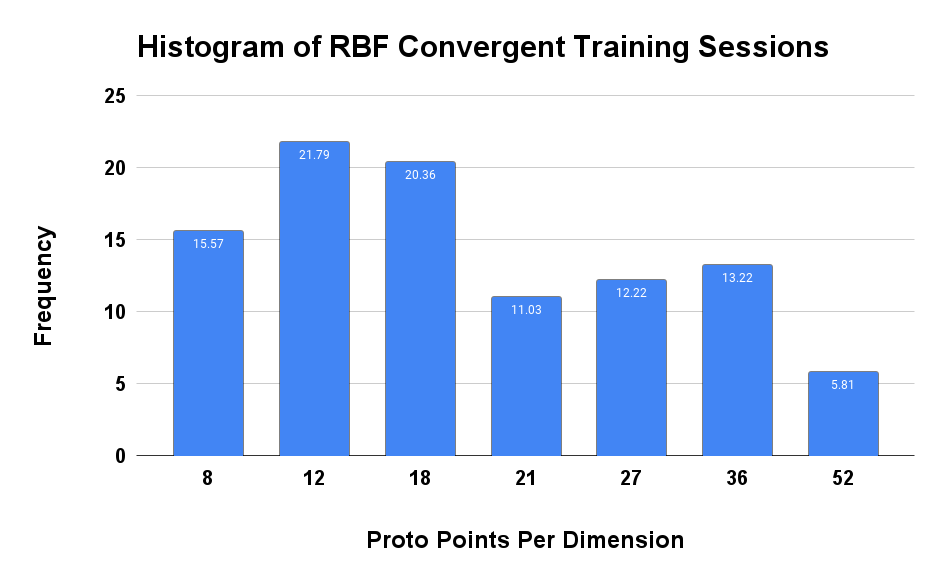
\includegraphics[scale=0.25]{histogram-rbf-convergent-training-sessions.png}
  \caption{Histogram of RBF Convergent Training Sessions.}
  \label{histogram_rbf_convergent_training_sessions}
\end{figure}

\begin{figure}[t]
  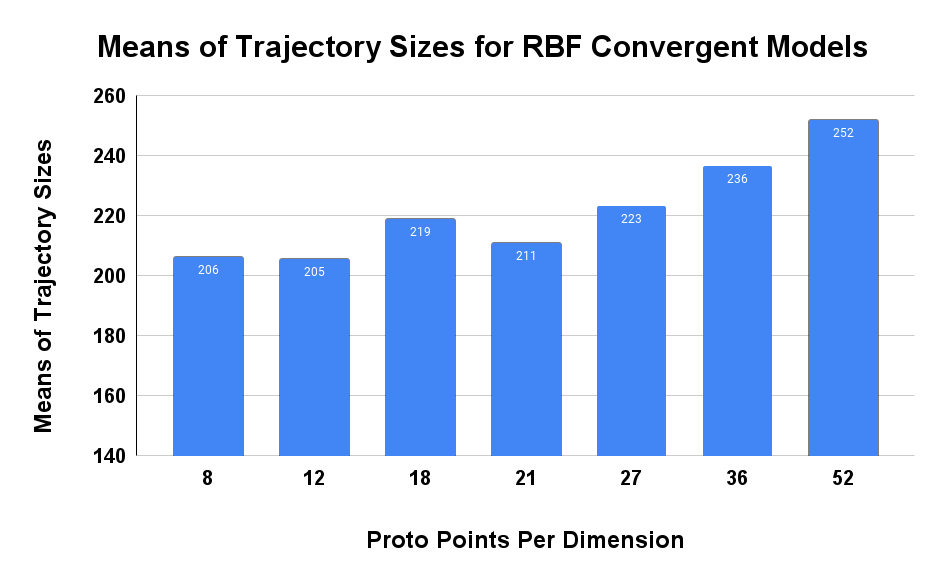
\includegraphics[scale=0.25]{means-of-trajectory-sizes-for-rbf-convergent-models.png}
  \caption{These represents the means of the averages of trajectories sizes obtained from each convergent model, considering the entire set of discoutings applied.}
  \label{means_of_trajectory_sizes_for_rbf_convergent_models}
\end{figure}


\section{Conclusions}
The results expose that RBF feature selection provides a better convergence rate (40.09\%) compared to polynomial feature selection (0.81\%), under
the same ranges of discountings applied ($\alpha$, $\gamma$ and $\epsilon$). The discounting selection having the best convergent rate for polynomial was trained in 4 sessions [\ref{polynomial-convergence-result}]
, while in RBF we have multiple discounting selections that were able to be trained on every session [\ref{rbf-convergence-result}]. It was proven empirically that convergence can be found for 
polynomial models although requiring more training sessions compared to RBF feature selections. A convergent polynomial model was trained with $\emph{polynomial dimension} = 2$
revealing that this problem can be solved with a model having 9 features, only. Comparing the models having the smallest trajectory sizes obtained in the 1000 simulations,
the RBF model trained with $\emph{proto points per dimension} = 8, \alpha = 0.025, \gamma = 0.95, \epsilon = 0.5 $ has completed the task with an average of 116.189 steps
while the polynomial model with $\emph{polynomial dimension} = 8, \alpha = 0.01, \gamma = 0.95, \epsilon = 0.75 $ has completed the task with an average of 112.728 steps.
This small difference reveals that both feature selections (RBF and Polynomials) under this same $TD(0)$ implementation has provided similar results to solve 
the proposed problem.         

\section{Limitations and Future Work}
It is out of the scope of this paper to evaluate theoretical arguments which explain why RBF feature selection has converged in more combinations of parameters 
and in less number of training sessions compared to polynomial feature selection. There are several areas of interest for future research. 
 In this experiment we have applied $TD(0)$ which is a particular implementation of
$TD(\lambda)$. Future work may generalize to $TD(\lambda)$ for convergence analysis. We built feature vectors $\mathbf{x}(s,a)$ 
and combined them linearly with the weight vector $\mathbf{w}$, which simplified the solution. There is an interest in evaluating wether exists convergence
improvement by adopting a neural network architecture instead. This research has fixed the number of episodes (500) in a training session, further investigations
may consider different numbers of episodes to understand which parametrization and feature selections may converge in fewer steps. We noticed that no convergence
 was obtained by larger values of $\alpha > 0.2$ for both RBF and polynomial features. Future executions should evaluate a set of $\alpha < 0.01$. 
 Although value function approximations has proven to provide satisfactory solutions, policy gradient theorem could be applied to pursue better convergence metrics.

\section{Appendix A: Source Code and Computing Resources}
The Semi-gradient Sarsa algorithm implemented in this research is public available for contributions (\href{https:\\github.com/mauriciocoder/mountain-car/tree/main}{GitHub}).
For this research, we used the computational power of three distinct servers running in parallel.
The first two servers, operating on the \texttt{x86\_64} architecture, is equipped with dual CPUs, each hosting two threads and supporting 64-bit CPU op-modes. 
Powered by the \texttt{AMD EPYC 7551 32-Core Processor}. These two servers runs on the Linux kernel version \texttt{5.15.0-1046-oracle}.
Our third server, underpinned by the \texttt{x86\_64} architecture, runs on \texttt{Intel(R) Xeon(R) CPU @ 2.20GHz}.
This server stands out with a unique cache setup, including a \texttt{55 MiB L3 cache}. The kernel version is \texttt{6.2.0-1019-gcp}
, and it belongs to the \texttt{Ubuntu} distribution with the release version \texttt{22.04.1}.

\bibliographystyle{abbrv}
\bibliography{bibliography.bib}

\newcommand{\ra}[1]{\renewcommand{\arraystretch}{#1}}  
\begin{table*}[t]
  \centering
  \ra{1.3}
  \begin{tabular}{@{}rrrr|r@{}}\toprule
  \multicolumn{5}{c}{\textbf{Highiest Convergent Models for Polynomial Feature Selection (from 10 training sessions)}}\\
  Alpha ($\alpha$) & Gamma ($\gamma$) & Dimension ($\emph{polynomial dimension}$) & Epsilon ($\epsilon$) & Convergent Training Sessions\\
  0.01 & 0.99 & 6 & 0.75 & 4\\
  0.01 & 1.0 & 6 & 0.75 & 3\\
  0.025 & 1.0 & 8 & 0.5 & 3\\
  0.025 & 0.9 & 10 & 0.5 & 3\\
  0.5 & 0.8 & 3 & 0.75 & 2\\
  0.075 & 0.99 & 4 & 0.75 & 2\\
  0.01 & 1.0 & 4 & 0.75 & 2\\
  0.01 & 0.9 & 4 & 0.5 & 2\\
  0.01 & 0.95 & 4 & 0.5 & 2\\
  0.01 & 1.0 & 5 & 0.75 & 2\\
  0.01 & 0.99 & 5 & 0.75 & 2\\
  0.05 & 0.99 & 5 & 0.75 & 2\\
  0.4 & 0.8 & 5 & 0.75 & 2\\
  0.5 & 0.8 & 5 & 0.5 & 2\\
  0.025 & 0.95 & 6 & 0.75 & 2\\
  0.05 & 0.99 & 7 & 0.5 & 2\\
  0.01 & 0.95 & 8 & 0.5 & 2\\
  0.01 & 0.9 & 8 & 0.5 & 2\\
  0.025 & 0.99 & 9 & 0.25 & 2\\
  0.01 & 0.95 & 9 & 0.5 & 2\\
  \bottomrule
  \end{tabular}
  \caption{Number of training sessions required for reaching convergence for polynomial feature selection models trained. We selected the highiest convergent models only.}
  \label{polynomial-convergence-result}
\end{table*}

\begin{table*}\centering
  \ra{1.3}
  \begin{tabular}{@{}rrrr|rrrrr@{}}\toprule
  \multicolumn{9}{c}{\textbf{Simulation results for Polynomial Feature Selection (from 1000 simulations)}}\\
  Alpha ($\alpha$) & Gamma ($\gamma$) & Dimension ($\emph{polynomial dimension}$) & Epsilon ($\epsilon$) & $Min$ & $Max$ & $\Delta$ & $Mean$ & $stdev$\\
  0.01 & 0.95 & 8 & 0.75 & 84 & 129 & 45 & 112.728 & 14.31\\
  0.01 & 0.95 & 9 & 0.75 & 112 & 132 & 20 & 115.517 & 3.25\\
  0.075 & 0.99 & 4 & 0.75 & 119 & 132 & 13 & 120.565 & 02.03\\
  0.01 & 0.9 & 8 & 0.5 & 92 & 139 & 47 & 124.689 & 12.32\\
  0.01 & 1.0 & 6 & 0.75 & 122 & 132 & 10 & 125.162 & 2.89\\
  0.01 & 0.9 & 8 & 0.5 & 85 & 180 & 95 & 126.212 & 24.70\\
  0.01 & 0.99 & 6 & 0.75 & 83 & 219 & 136 & 131.896 & 37.79\\
  0.01 & 1.0 & 6 & 0.75 & 84 & 261 & 177 & 134.657 & 48.22\\
  0.025 & 0.99 & 9 & 0.5 & 107 & 150 & 43 & 138.051 & 10.91\\
  0.1 & 1.0 & 3 & 0.75 & 115 & 211 & 96 & 138.573 & 35.47\\
  0.01 & 0.95 & 9 & 0.5 & 83 & 259 & 176 & 139.247 & 39.37\\
  0.125 & 1.0 & 4 & 0.75 & 83 & 244 & 161 & 139.843 & 43.88\\
  0.025 & 1.0 & 8 & 0.5 & 87 & 259 & 172 & 140.994 & 36.84\\
  0.075 & 1.0 & 3 & 0.75 & 83 & 261 & 178 & 141.362 & 42.93\\
  0.05 & 1.0 & 6 & 0.5 & 134 & 211 & 77 & 141.779 & 19.18\\
  0.025 & 0.99 & 10 & 0.75 & 83 & 235 & 152 & 142.174 & 41.17\\
  0.01 & 1.0 & 5 & 0.75 & 83 & 274 & 191 & 142.181 & 46.08\\
  0.025 & 0.99 & 10 & 0.25 & 112 & 220 & 108 & 144.271 & 27.75\\
  0.05 & 0.99 & 5 & 0.75 & 83 & 265 & 182 & 144.325 & 46.20\\
  0.175 & 0.99 & 3 & 0.75 & 83 & 203 & 120 & 144.669 & 38.36\\
  0.05 & 0.9 & 7 & 0.5 & 111 & 211 & 100 & 145.931 & 30.48\\
  \bottomrule
  \end{tabular}
  \caption{Simulation results with trajectory sizes for polynomial feature selection (from 1000 simulations). Table sorted by ascending mean of trajectory sizes and filtered by models with better means. }
  \label{polynomial-simulation-result}
\end{table*}

\begin{table*}
  \centering
  \ra{1.3}
  \begin{tabular}{@{}rrrr|r@{}}\toprule
  \multicolumn{5}{c}{\textbf{Convergent Models for RBF Feature Selection (from 10 training sessions)}}\\
  Alpha ($\alpha$) & Gamma ($\gamma$) & Points ($\emph{proto points per dimension}$) & Epsilon ($\epsilon$) & Convergent Training Sessions\\
  0.75 & 1.0 & 12 & 0.25 & 10\\
  0.1 & 0.99 & 12 & 0.25 & 10\\
  0.2 & 1.0 & 36 & 0.75 & 10\\
  0.025 & 0.95 & 12 & 0.5 & 10\\
  0.75 & 0.99 & 18 & 0.75 & 10\\
  0.75 & 0.95 & 18 & 0.5 & 10\\
  0.1 & 0.8 & 18 & 0.5 & 10\\
  0.2 & 0.95 & 18 & 0.75 & 10\\
  0.025 & 0.9 & 12 & 0.75 & 10\\
  0.125 & 0.8 & 12 & 0.25 & 10\\
  0.75 & 0.95 & 12 & 0.75 & 10\\
  0.05 & 0.9 & 12 & 0.75 & 10\\
  0.15 & 0.9 & 12 & 0.25 & 10\\
  0.75 & 0.8 & 18 & 0.75 & 10\\
  0.1 & 0.8 & 18 & 0.75 & 10\\
  0.15 & 1.0 & 12 & 0.25 & 10\\
  0.2 & 0.9 & 18 & 0.25 & 10\\
  0.125 & 0.95 & 12 & 0.75 & 10\\
  0.05 & 1.0 & 12 & 0.5 & 10\\
  0.025 & 0.95 & 12 & 0.75 & 10\\
  0.01 & 0.8 & 8 & 0.75 & 10\\
  0.025 & 0.95 & 18 & 0.75 & 10\\
  0.05 & 0.99 & 8 & 0.5 & 10\\
  0.05 & 0.95 & 12 & 0.75 & 10\\
  0.75 & 0.9 & 12 & 0.25 & 10\\
  0.75 & 0.9 & 12 & 0.5 & 10\\
  0.01 & 0.8 & 12 & 0.75 & 10\\
  0.75 & 0.9 & 18 & 0.5 & 10\\
  0.01 & 0.9 & 8 & 0.75 & 10\\
  0.125 & 0.99 & 12 & 0.5 & 10\\
  0.75 & 0.99 & 12 & 0.5 & 10\\
  \bottomrule
  \end{tabular}
  \caption{Number of training sessions required for reaching convergence for RBF feature selection models trained.}
  \label{rbf-convergence-result}
\end{table*}

\begin{table*}\centering
  \ra{1.3}
  \begin{tabular}{@{}rrrr|rrrrr@{}}\toprule
  \multicolumn{9}{c}{\textbf{Simulation results for RBF Feature Selection (from 1000 simulations)}}\\
  Alpha ($\alpha$) & Gamma ($\gamma$) & Dimension ($\emph{proto points per dimension}$) & Epsilon ($\epsilon$) & $Min$ & $Max$ & $\Delta$ & $Mean$ & $stdev$\\
  0.025 & 0.95 & 8 & 0.5 & 110 & 133 & 23 & 116.189 & 5.13\\
  0.01 & 0.99 & 8 & 0.5 & 113 & 125 & 12 & 117.502 & 3.45\\
  0.125 & 1 & 8 & 0.25 & 111 & 133 & 22 & 118.231 & 5.16\\
  0.05 & 0.99 & 8 & 0.5 & 113 & 133 & 20 & 119.369 & 4.37\\
  0.01 & 0.8 & 8 & 0.5 & 90 & 228 & 138 & 119.376 & 20.62\\
  0.01 & 0.8 & 8 & 0.25 & 115 & 133 & 18 & 120.07 & 4.51\\
  0.025 & 0.8 & 8 & 0.5 & 114 & 202 & 88 & 120.105 & 13.01\\
  0.01 & 0.9 & 12 & 0.75 & 116 & 129 & 13 & 120.285 & 3.31\\
  0.075 & 1 & 8 & 0.5 & 117 & 133 & 16 & 120.68 & 4.01\\
  0.1 & 1 & 8 & 0.25 & 109 & 242 & 133 & 121.016 & 24.35\\
  0.2 & 0.8 & 8 & 0.25 & 116 & 130 & 14 & 122.161 & 4.91\\
  0.175 & 0.95 & 12 & 0.25 & 96 & 198 & 102 & 122.938 & 14.56\\
  0.1 & 1 & 8 & 0.25 & 88 & 144 & 56 & 123.212 & 18.00\\
  0.01 & 0.9 & 8 & 0.5 & 121 & 233 & 112 & 124.317 & 9.83\\
  0.01 & 0.9 & 12 & 0.75 & 89 & 197 & 108 & 126.354 & 25.45\\
  0.025 & 0.9 & 12 & 0.5 & 96 & 191 & 95 & 126.65 & 17.24\\
  0.025 & 0.95 & 8 & 0.25 & 121 & 389 & 268 & 127.173 & 24.18\\
  0.025 & 0.9 & 8 & 0.25 & 112 & 183 & 71 & 129.03 & 25.17\\
  0.05 & 0.99 & 8 & 0.75 & 110 & 158 & 48 & 129.325 & 14.20\\
  0.025 & 0.8 & 12 & 0.75 & 85 & 195 & 110 & 130.392 & 29.74\\
  0.01 & 1 & 8 & 0.75 & 105 & 214 & 109 & 130.831 & 21.04\\
  0.075 & 0.99 & 8 & 0.25 & 111 & 173 & 62 & 130.937 & 18.18\\
  0.1 & 1 & 8 & 0.5 & 93 & 157 & 64 & 131.359 & 21.97\\
  0.2 & 0.9 & 8 & 0.25 & 122 & 265 & 143 & 131.442 & 18.77\\
  0.1 & 0.99 & 8 & 0.75 & 129 & 137 & 8 & 132.594 & 1.67\\
  0.05 & 0.99 & 8 & 0.5 & 128 & 138 & 10 & 132.98 & 2.27\\
  0.05 & 0.8 & 12 & 0.5 & 96 & 191 & 95 & 133.978 & 18.24\\
  0.125 & 0.99 & 12 & 0.5 & 114 & 185 & 71 & 134.974 & 22.77\\
  0.1 & 1 & 8 & 0.25 & 85 & 205 & 120 & 135.421 & 20.05\\
  0.125 & 0.8 & 18 & 0.25 & 95 & 204 & 109 & 135.468 & 21.53\\
  \bottomrule
  \end{tabular}
  \caption{Simulation results with trajectory sizes for RBF feature selection (from 1000 simulations). Table sorted by ascending mean of trajectory sizes and filtered by models with better means.}
  \label{rbf-simulation-result}
\end{table*}


\end{document}
